% Created by tikzDevice version 0.10.1 on 2018-02-19 11:27:10
% !TEX encoding = UTF-8 Unicode
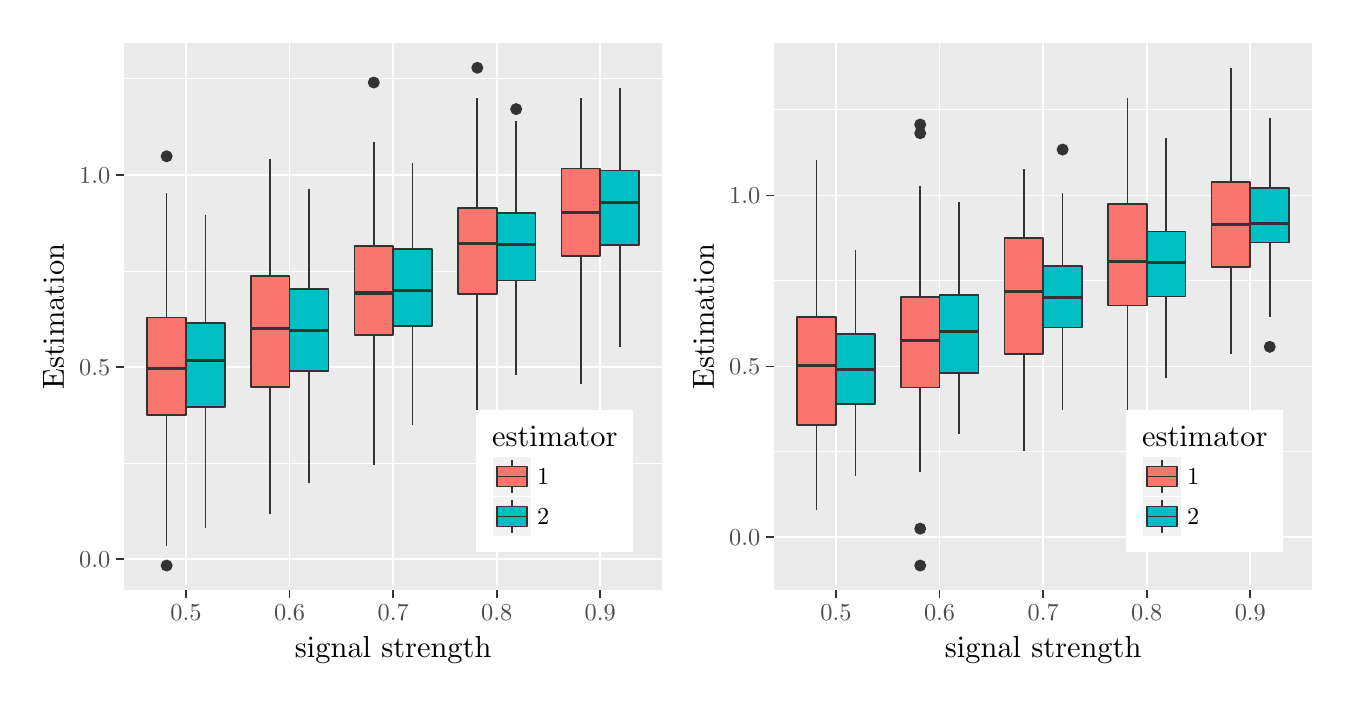
\begin{tikzpicture}[x=1pt,y=1pt]
\definecolor{fillColor}{RGB}{255,255,255}
\path[use as bounding box,fill=fillColor,fill opacity=0.00] (0,0) rectangle (469.76,234.88);
\begin{scope}
\path[clip] (  0.00,  0.00) rectangle (234.88,234.88);
\definecolor{drawColor}{RGB}{255,255,255}
\definecolor{fillColor}{RGB}{255,255,255}

\path[draw=drawColor,line width= 0.6pt,line join=round,line cap=round,fill=fillColor] (  0.00,  0.00) rectangle (234.88,234.88);
\end{scope}
\begin{scope}
\path[clip] ( 34.77, 31.53) rectangle (229.38,229.38);
\definecolor{fillColor}{gray}{0.92}

\path[fill=fillColor] ( 34.77, 31.53) rectangle (229.38,229.38);
\definecolor{drawColor}{RGB}{255,255,255}

\path[draw=drawColor,line width= 0.3pt,line join=round] ( 34.77, 77.50) --
	(229.38, 77.50);

\path[draw=drawColor,line width= 0.3pt,line join=round] ( 34.77,146.97) --
	(229.38,146.97);

\path[draw=drawColor,line width= 0.3pt,line join=round] ( 34.77,216.44) --
	(229.38,216.44);

\path[draw=drawColor,line width= 0.6pt,line join=round] ( 34.77, 42.77) --
	(229.38, 42.77);

\path[draw=drawColor,line width= 0.6pt,line join=round] ( 34.77,112.24) --
	(229.38,112.24);

\path[draw=drawColor,line width= 0.6pt,line join=round] ( 34.77,181.70) --
	(229.38,181.70);

\path[draw=drawColor,line width= 0.6pt,line join=round] ( 57.22, 31.53) --
	( 57.22,229.38);

\path[draw=drawColor,line width= 0.6pt,line join=round] ( 94.65, 31.53) --
	( 94.65,229.38);

\path[draw=drawColor,line width= 0.6pt,line join=round] (132.07, 31.53) --
	(132.07,229.38);

\path[draw=drawColor,line width= 0.6pt,line join=round] (169.50, 31.53) --
	(169.50,229.38);

\path[draw=drawColor,line width= 0.6pt,line join=round] (206.92, 31.53) --
	(206.92,229.38);
\definecolor{drawColor}{gray}{0.20}
\definecolor{fillColor}{gray}{0.20}

\path[draw=drawColor,line width= 0.4pt,line join=round,line cap=round,fill=fillColor] ( 50.21,188.41) circle (  1.96);

\path[draw=drawColor,line width= 0.4pt,line join=round,line cap=round,fill=fillColor] ( 50.21, 40.52) circle (  1.96);

\path[draw=drawColor,line width= 0.6pt,line join=round] ( 50.21,130.19) -- ( 50.21,175.29);

\path[draw=drawColor,line width= 0.6pt,line join=round] ( 50.21, 94.84) -- ( 50.21, 47.45);
\definecolor{fillColor}{RGB}{248,118,109}

\path[draw=drawColor,line width= 0.6pt,line join=round,line cap=round,fill=fillColor] ( 43.19,130.19) --
	( 43.19, 94.84) --
	( 57.22, 94.84) --
	( 57.22,130.19) --
	( 43.19,130.19) --
	cycle;

\path[draw=drawColor,line width= 1.1pt,line join=round] ( 43.19,111.62) -- ( 57.22,111.62);

\path[draw=drawColor,line width= 0.6pt,line join=round] ( 64.24,128.06) -- ( 64.24,167.11);

\path[draw=drawColor,line width= 0.6pt,line join=round] ( 64.24, 97.88) -- ( 64.24, 53.91);
\definecolor{fillColor}{RGB}{0,191,196}

\path[draw=drawColor,line width= 0.6pt,line join=round,line cap=round,fill=fillColor] ( 57.22,128.06) --
	( 57.22, 97.88) --
	( 71.26, 97.88) --
	( 71.26,128.06) --
	( 57.22,128.06) --
	cycle;

\path[draw=drawColor,line width= 1.1pt,line join=round] ( 57.22,114.72) -- ( 71.26,114.72);

\path[draw=drawColor,line width= 0.6pt,line join=round] ( 87.63,145.09) -- ( 87.63,187.26);

\path[draw=drawColor,line width= 0.6pt,line join=round] ( 87.63,105.04) -- ( 87.63, 59.21);
\definecolor{fillColor}{RGB}{248,118,109}

\path[draw=drawColor,line width= 0.6pt,line join=round,line cap=round,fill=fillColor] ( 80.61,145.09) --
	( 80.61,105.04) --
	( 94.65,105.04) --
	( 94.65,145.09) --
	( 80.61,145.09) --
	cycle;

\path[draw=drawColor,line width= 1.1pt,line join=round] ( 80.61,126.09) -- ( 94.65,126.09);

\path[draw=drawColor,line width= 0.6pt,line join=round] (101.66,140.54) -- (101.66,176.76);

\path[draw=drawColor,line width= 0.6pt,line join=round] (101.66,110.76) -- (101.66, 70.31);
\definecolor{fillColor}{RGB}{0,191,196}

\path[draw=drawColor,line width= 0.6pt,line join=round,line cap=round,fill=fillColor] ( 94.65,140.54) --
	( 94.65,110.76) --
	(108.68,110.76) --
	(108.68,140.54) --
	( 94.65,140.54) --
	cycle;

\path[draw=drawColor,line width= 1.1pt,line join=round] ( 94.65,125.46) -- (108.68,125.46);
\definecolor{fillColor}{gray}{0.20}

\path[draw=drawColor,line width= 0.4pt,line join=round,line cap=round,fill=fillColor] (125.06,215.05) circle (  1.96);

\path[draw=drawColor,line width= 0.6pt,line join=round] (125.06,155.99) -- (125.06,193.41);

\path[draw=drawColor,line width= 0.6pt,line join=round] (125.06,123.93) -- (125.06, 76.79);
\definecolor{fillColor}{RGB}{248,118,109}

\path[draw=drawColor,line width= 0.6pt,line join=round,line cap=round,fill=fillColor] (118.04,155.99) --
	(118.04,123.93) --
	(132.07,123.93) --
	(132.07,155.99) --
	(118.04,155.99) --
	cycle;

\path[draw=drawColor,line width= 1.1pt,line join=round] (118.04,139.00) -- (132.07,139.00);

\path[draw=drawColor,line width= 0.6pt,line join=round] (139.09,154.93) -- (139.09,185.82);

\path[draw=drawColor,line width= 0.6pt,line join=round] (139.09,127.01) -- (139.09, 91.20);
\definecolor{fillColor}{RGB}{0,191,196}

\path[draw=drawColor,line width= 0.6pt,line join=round,line cap=round,fill=fillColor] (132.07,154.93) --
	(132.07,127.01) --
	(146.11,127.01) --
	(146.11,154.93) --
	(132.07,154.93) --
	cycle;

\path[draw=drawColor,line width= 1.1pt,line join=round] (132.07,139.94) -- (146.11,139.94);
\definecolor{fillColor}{gray}{0.20}

\path[draw=drawColor,line width= 0.4pt,line join=round,line cap=round,fill=fillColor] (162.48,220.38) circle (  1.96);

\path[draw=drawColor,line width= 0.6pt,line join=round] (162.48,169.63) -- (162.48,209.61);

\path[draw=drawColor,line width= 0.6pt,line join=round] (162.48,138.56) -- (162.48, 96.73);
\definecolor{fillColor}{RGB}{248,118,109}

\path[draw=drawColor,line width= 0.6pt,line join=round,line cap=round,fill=fillColor] (155.46,169.63) --
	(155.46,138.56) --
	(169.50,138.56) --
	(169.50,169.63) --
	(155.46,169.63) --
	cycle;

\path[draw=drawColor,line width= 1.1pt,line join=round] (155.46,156.92) -- (169.50,156.92);
\definecolor{fillColor}{gray}{0.20}

\path[draw=drawColor,line width= 0.4pt,line join=round,line cap=round,fill=fillColor] (176.51,205.46) circle (  1.96);

\path[draw=drawColor,line width= 0.6pt,line join=round] (176.51,167.84) -- (176.51,201.10);

\path[draw=drawColor,line width= 0.6pt,line join=round] (176.51,143.56) -- (176.51,109.28);
\definecolor{fillColor}{RGB}{0,191,196}

\path[draw=drawColor,line width= 0.6pt,line join=round,line cap=round,fill=fillColor] (169.50,167.84) --
	(169.50,143.56) --
	(183.53,143.56) --
	(183.53,167.84) --
	(169.50,167.84) --
	cycle;

\path[draw=drawColor,line width= 1.1pt,line join=round] (169.50,156.56) -- (183.53,156.56);

\path[draw=drawColor,line width= 0.6pt,line join=round] (199.91,183.99) -- (199.91,209.29);

\path[draw=drawColor,line width= 0.6pt,line join=round] (199.91,152.49) -- (199.91,105.98);
\definecolor{fillColor}{RGB}{248,118,109}

\path[draw=drawColor,line width= 0.6pt,line join=round,line cap=round,fill=fillColor] (192.89,183.99) --
	(192.89,152.49) --
	(206.92,152.49) --
	(206.92,183.99) --
	(192.89,183.99) --
	cycle;

\path[draw=drawColor,line width= 1.1pt,line join=round] (192.89,167.97) -- (206.92,167.97);

\path[draw=drawColor,line width= 0.6pt,line join=round] (213.94,183.32) -- (213.94,213.00);

\path[draw=drawColor,line width= 0.6pt,line join=round] (213.94,156.27) -- (213.94,119.65);
\definecolor{fillColor}{RGB}{0,191,196}

\path[draw=drawColor,line width= 0.6pt,line join=round,line cap=round,fill=fillColor] (206.92,183.32) --
	(206.92,156.27) --
	(220.96,156.27) --
	(220.96,183.32) --
	(206.92,183.32) --
	cycle;

\path[draw=drawColor,line width= 1.1pt,line join=round] (206.92,171.64) -- (220.96,171.64);
\end{scope}
\begin{scope}
\path[clip] (  0.00,  0.00) rectangle (469.76,234.88);
\definecolor{drawColor}{gray}{0.30}

\node[text=drawColor,anchor=base east,inner sep=0pt, outer sep=0pt, scale=  0.88] at ( 29.82, 39.74) {0.0};

\node[text=drawColor,anchor=base east,inner sep=0pt, outer sep=0pt, scale=  0.88] at ( 29.82,109.21) {0.5};

\node[text=drawColor,anchor=base east,inner sep=0pt, outer sep=0pt, scale=  0.88] at ( 29.82,178.67) {1.0};
\end{scope}
\begin{scope}
\path[clip] (  0.00,  0.00) rectangle (469.76,234.88);
\definecolor{drawColor}{gray}{0.20}

\path[draw=drawColor,line width= 0.6pt,line join=round] ( 32.02, 42.77) --
	( 34.77, 42.77);

\path[draw=drawColor,line width= 0.6pt,line join=round] ( 32.02,112.24) --
	( 34.77,112.24);

\path[draw=drawColor,line width= 0.6pt,line join=round] ( 32.02,181.70) --
	( 34.77,181.70);
\end{scope}
\begin{scope}
\path[clip] (  0.00,  0.00) rectangle (469.76,234.88);
\definecolor{drawColor}{gray}{0.20}

\path[draw=drawColor,line width= 0.6pt,line join=round] ( 57.22, 28.78) --
	( 57.22, 31.53);

\path[draw=drawColor,line width= 0.6pt,line join=round] ( 94.65, 28.78) --
	( 94.65, 31.53);

\path[draw=drawColor,line width= 0.6pt,line join=round] (132.07, 28.78) --
	(132.07, 31.53);

\path[draw=drawColor,line width= 0.6pt,line join=round] (169.50, 28.78) --
	(169.50, 31.53);

\path[draw=drawColor,line width= 0.6pt,line join=round] (206.92, 28.78) --
	(206.92, 31.53);
\end{scope}
\begin{scope}
\path[clip] (  0.00,  0.00) rectangle (469.76,234.88);
\definecolor{drawColor}{gray}{0.30}

\node[text=drawColor,anchor=base,inner sep=0pt, outer sep=0pt, scale=  0.88] at ( 57.22, 20.52) {0.5};

\node[text=drawColor,anchor=base,inner sep=0pt, outer sep=0pt, scale=  0.88] at ( 94.65, 20.52) {0.6};

\node[text=drawColor,anchor=base,inner sep=0pt, outer sep=0pt, scale=  0.88] at (132.07, 20.52) {0.7};

\node[text=drawColor,anchor=base,inner sep=0pt, outer sep=0pt, scale=  0.88] at (169.50, 20.52) {0.8};

\node[text=drawColor,anchor=base,inner sep=0pt, outer sep=0pt, scale=  0.88] at (206.92, 20.52) {0.9};
\end{scope}
\begin{scope}
\path[clip] (  0.00,  0.00) rectangle (469.76,234.88);
\definecolor{drawColor}{RGB}{0,0,0}

\node[text=drawColor,anchor=base,inner sep=0pt, outer sep=0pt, scale=  1.10] at (132.07,  7.44) {signal strength};
\end{scope}
\begin{scope}
\path[clip] (  0.00,  0.00) rectangle (469.76,234.88);
\definecolor{drawColor}{RGB}{0,0,0}

\node[text=drawColor,rotate= 90.00,anchor=base,inner sep=0pt, outer sep=0pt, scale=  1.10] at ( 13.08,130.45) {Estimation};
\end{scope}
\begin{scope}
\path[clip] (  0.00,  0.00) rectangle (469.76,234.88);
\definecolor{fillColor}{RGB}{255,255,255}

\path[fill=fillColor] (162.11, 45.36) rectangle (218.80, 96.84);
\end{scope}
\begin{scope}
\path[clip] (  0.00,  0.00) rectangle (469.76,234.88);
\definecolor{drawColor}{RGB}{0,0,0}

\node[text=drawColor,anchor=base west,inner sep=0pt, outer sep=0pt, scale=  1.10] at (167.80, 83.57) {estimator};
\end{scope}
\begin{scope}
\path[clip] (  0.00,  0.00) rectangle (469.76,234.88);
\definecolor{drawColor}{RGB}{255,255,255}
\definecolor{fillColor}{gray}{0.95}

\path[draw=drawColor,line width= 0.6pt,line join=round,line cap=round,fill=fillColor] (167.80, 65.51) rectangle (182.26, 79.96);
\end{scope}
\begin{scope}
\path[clip] (  0.00,  0.00) rectangle (469.76,234.88);
\definecolor{drawColor}{gray}{0.20}

\path[draw=drawColor,line width= 0.6pt,line join=round,line cap=round] (175.03, 66.95) --
	(175.03, 69.12);

\path[draw=drawColor,line width= 0.6pt,line join=round,line cap=round] (175.03, 76.35) --
	(175.03, 78.51);
\definecolor{fillColor}{RGB}{248,118,109}

\path[draw=drawColor,line width= 0.6pt,line join=round,line cap=round,fill=fillColor] (169.61, 69.12) rectangle (180.45, 76.35);

\path[draw=drawColor,line width= 0.6pt,line join=round,line cap=round] (169.61, 72.73) --
	(180.45, 72.73);
\end{scope}
\begin{scope}
\path[clip] (  0.00,  0.00) rectangle (469.76,234.88);
\definecolor{drawColor}{RGB}{255,255,255}
\definecolor{fillColor}{gray}{0.95}

\path[draw=drawColor,line width= 0.6pt,line join=round,line cap=round,fill=fillColor] (167.80, 51.05) rectangle (182.26, 65.51);
\end{scope}
\begin{scope}
\path[clip] (  0.00,  0.00) rectangle (469.76,234.88);
\definecolor{drawColor}{gray}{0.20}

\path[draw=drawColor,line width= 0.6pt,line join=round,line cap=round] (175.03, 52.50) --
	(175.03, 54.66);

\path[draw=drawColor,line width= 0.6pt,line join=round,line cap=round] (175.03, 61.89) --
	(175.03, 64.06);
\definecolor{fillColor}{RGB}{0,191,196}

\path[draw=drawColor,line width= 0.6pt,line join=round,line cap=round,fill=fillColor] (169.61, 54.66) rectangle (180.45, 61.89);

\path[draw=drawColor,line width= 0.6pt,line join=round,line cap=round] (169.61, 58.28) --
	(180.45, 58.28);
\end{scope}
\begin{scope}
\path[clip] (  0.00,  0.00) rectangle (469.76,234.88);
\definecolor{drawColor}{RGB}{0,0,0}

\node[text=drawColor,anchor=base west,inner sep=0pt, outer sep=0pt, scale=  0.88] at (184.06, 69.70) {1};
\end{scope}
\begin{scope}
\path[clip] (  0.00,  0.00) rectangle (469.76,234.88);
\definecolor{drawColor}{RGB}{0,0,0}

\node[text=drawColor,anchor=base west,inner sep=0pt, outer sep=0pt, scale=  0.88] at (184.06, 55.25) {2};
\end{scope}
\begin{scope}
\path[clip] (234.88,  0.00) rectangle (469.76,234.88);
\definecolor{drawColor}{RGB}{255,255,255}
\definecolor{fillColor}{RGB}{255,255,255}

\path[draw=drawColor,line width= 0.6pt,line join=round,line cap=round,fill=fillColor] (234.88,  0.00) rectangle (469.76,234.88);
\end{scope}
\begin{scope}
\path[clip] (269.65, 31.53) rectangle (464.26,229.38);
\definecolor{fillColor}{gray}{0.92}

\path[fill=fillColor] (269.65, 31.53) rectangle (464.26,229.38);
\definecolor{drawColor}{RGB}{255,255,255}

\path[draw=drawColor,line width= 0.3pt,line join=round] (269.65, 81.61) --
	(464.26, 81.61);

\path[draw=drawColor,line width= 0.3pt,line join=round] (269.65,143.39) --
	(464.26,143.39);

\path[draw=drawColor,line width= 0.3pt,line join=round] (269.65,205.16) --
	(464.26,205.16);

\path[draw=drawColor,line width= 0.6pt,line join=round] (269.65, 50.72) --
	(464.26, 50.72);

\path[draw=drawColor,line width= 0.6pt,line join=round] (269.65,112.50) --
	(464.26,112.50);

\path[draw=drawColor,line width= 0.6pt,line join=round] (269.65,174.27) --
	(464.26,174.27);

\path[draw=drawColor,line width= 0.6pt,line join=round] (292.10, 31.53) --
	(292.10,229.38);

\path[draw=drawColor,line width= 0.6pt,line join=round] (329.53, 31.53) --
	(329.53,229.38);

\path[draw=drawColor,line width= 0.6pt,line join=round] (366.95, 31.53) --
	(366.95,229.38);

\path[draw=drawColor,line width= 0.6pt,line join=round] (404.38, 31.53) --
	(404.38,229.38);

\path[draw=drawColor,line width= 0.6pt,line join=round] (441.80, 31.53) --
	(441.80,229.38);
\definecolor{drawColor}{gray}{0.20}

\path[draw=drawColor,line width= 0.6pt,line join=round] (285.08,130.34) -- (285.08,186.96);

\path[draw=drawColor,line width= 0.6pt,line join=round] (285.08, 91.36) -- (285.08, 60.62);
\definecolor{fillColor}{RGB}{248,118,109}

\path[draw=drawColor,line width= 0.6pt,line join=round,line cap=round,fill=fillColor] (278.07,130.34) --
	(278.07, 91.36) --
	(292.10, 91.36) --
	(292.10,130.34) --
	(278.07,130.34) --
	cycle;

\path[draw=drawColor,line width= 1.1pt,line join=round] (278.07,112.76) -- (292.10,112.76);

\path[draw=drawColor,line width= 0.6pt,line join=round] (299.12,124.12) -- (299.12,154.47);

\path[draw=drawColor,line width= 0.6pt,line join=round] (299.12, 98.96) -- (299.12, 72.97);
\definecolor{fillColor}{RGB}{0,191,196}

\path[draw=drawColor,line width= 0.6pt,line join=round,line cap=round,fill=fillColor] (292.10,124.12) --
	(292.10, 98.96) --
	(306.13, 98.96) --
	(306.13,124.12) --
	(292.10,124.12) --
	cycle;

\path[draw=drawColor,line width= 1.1pt,line join=round] (292.10,111.39) -- (306.13,111.39);
\definecolor{fillColor}{gray}{0.20}

\path[draw=drawColor,line width= 0.4pt,line join=round,line cap=round,fill=fillColor] (322.51, 40.52) circle (  1.96);

\path[draw=drawColor,line width= 0.4pt,line join=round,line cap=round,fill=fillColor] (322.51, 53.84) circle (  1.96);

\path[draw=drawColor,line width= 0.4pt,line join=round,line cap=round,fill=fillColor] (322.51,199.88) circle (  1.96);

\path[draw=drawColor,line width= 0.4pt,line join=round,line cap=round,fill=fillColor] (322.51,196.74) circle (  1.96);

\path[draw=drawColor,line width= 0.6pt,line join=round] (322.51,137.48) -- (322.51,177.73);

\path[draw=drawColor,line width= 0.6pt,line join=round] (322.51,104.81) -- (322.51, 74.22);
\definecolor{fillColor}{RGB}{248,118,109}

\path[draw=drawColor,line width= 0.6pt,line join=round,line cap=round,fill=fillColor] (315.49,137.48) --
	(315.49,104.81) --
	(329.53,104.81) --
	(329.53,137.48) --
	(315.49,137.48) --
	cycle;

\path[draw=drawColor,line width= 1.1pt,line join=round] (315.49,121.86) -- (329.53,121.86);

\path[draw=drawColor,line width= 0.6pt,line join=round] (336.54,138.17) -- (336.54,171.94);

\path[draw=drawColor,line width= 0.6pt,line join=round] (336.54,110.02) -- (336.54, 87.94);
\definecolor{fillColor}{RGB}{0,191,196}

\path[draw=drawColor,line width= 0.6pt,line join=round,line cap=round,fill=fillColor] (329.53,138.17) --
	(329.53,110.02) --
	(343.56,110.02) --
	(343.56,138.17) --
	(329.53,138.17) --
	cycle;

\path[draw=drawColor,line width= 1.1pt,line join=round] (329.53,125.02) -- (343.56,125.02);

\path[draw=drawColor,line width= 0.6pt,line join=round] (359.93,158.93) -- (359.93,183.70);

\path[draw=drawColor,line width= 0.6pt,line join=round] (359.93,117.04) -- (359.93, 82.09);
\definecolor{fillColor}{RGB}{248,118,109}

\path[draw=drawColor,line width= 0.6pt,line join=round,line cap=round,fill=fillColor] (352.92,158.93) --
	(352.92,117.04) --
	(366.95,117.04) --
	(366.95,158.93) --
	(352.92,158.93) --
	cycle;

\path[draw=drawColor,line width= 1.1pt,line join=round] (352.92,139.70) -- (366.95,139.70);
\definecolor{fillColor}{gray}{0.20}

\path[draw=drawColor,line width= 0.4pt,line join=round,line cap=round,fill=fillColor] (373.97,190.83) circle (  1.96);

\path[draw=drawColor,line width= 0.6pt,line join=round] (373.97,148.87) -- (373.97,175.19);

\path[draw=drawColor,line width= 0.6pt,line join=round] (373.97,126.56) -- (373.97, 96.56);
\definecolor{fillColor}{RGB}{0,191,196}

\path[draw=drawColor,line width= 0.6pt,line join=round,line cap=round,fill=fillColor] (366.95,148.87) --
	(366.95,126.56) --
	(380.98,126.56) --
	(380.98,148.87) --
	(366.95,148.87) --
	cycle;

\path[draw=drawColor,line width= 1.1pt,line join=round] (366.95,137.31) -- (380.98,137.31);

\path[draw=drawColor,line width= 0.6pt,line join=round] (397.36,171.20) -- (397.36,209.57);

\path[draw=drawColor,line width= 0.6pt,line join=round] (397.36,134.47) -- (397.36, 84.98);
\definecolor{fillColor}{RGB}{248,118,109}

\path[draw=drawColor,line width= 0.6pt,line join=round,line cap=round,fill=fillColor] (390.34,171.20) --
	(390.34,134.47) --
	(404.38,134.47) --
	(404.38,171.20) --
	(390.34,171.20) --
	cycle;

\path[draw=drawColor,line width= 1.1pt,line join=round] (390.34,150.37) -- (404.38,150.37);

\path[draw=drawColor,line width= 0.6pt,line join=round] (411.39,161.21) -- (411.39,194.99);

\path[draw=drawColor,line width= 0.6pt,line join=round] (411.39,137.75) -- (411.39,108.45);
\definecolor{fillColor}{RGB}{0,191,196}

\path[draw=drawColor,line width= 0.6pt,line join=round,line cap=round,fill=fillColor] (404.38,161.21) --
	(404.38,137.75) --
	(418.41,137.75) --
	(418.41,161.21) --
	(404.38,161.21) --
	cycle;

\path[draw=drawColor,line width= 1.1pt,line join=round] (404.38,150.16) -- (418.41,150.16);

\path[draw=drawColor,line width= 0.6pt,line join=round] (434.78,179.14) -- (434.78,220.38);

\path[draw=drawColor,line width= 0.6pt,line join=round] (434.78,148.46) -- (434.78,117.11);
\definecolor{fillColor}{RGB}{248,118,109}

\path[draw=drawColor,line width= 0.6pt,line join=round,line cap=round,fill=fillColor] (427.77,179.14) --
	(427.77,148.46) --
	(441.80,148.46) --
	(441.80,179.14) --
	(427.77,179.14) --
	cycle;

\path[draw=drawColor,line width= 1.1pt,line join=round] (427.77,163.70) -- (441.80,163.70);
\definecolor{fillColor}{gray}{0.20}

\path[draw=drawColor,line width= 0.4pt,line join=round,line cap=round,fill=fillColor] (448.82,119.55) circle (  1.96);

\path[draw=drawColor,line width= 0.6pt,line join=round] (448.82,176.94) -- (448.82,202.12);

\path[draw=drawColor,line width= 0.6pt,line join=round] (448.82,157.31) -- (448.82,130.16);
\definecolor{fillColor}{RGB}{0,191,196}

\path[draw=drawColor,line width= 0.6pt,line join=round,line cap=round,fill=fillColor] (441.80,176.94) --
	(441.80,157.31) --
	(455.83,157.31) --
	(455.83,176.94) --
	(441.80,176.94) --
	cycle;

\path[draw=drawColor,line width= 1.1pt,line join=round] (441.80,164.19) -- (455.83,164.19);
\end{scope}
\begin{scope}
\path[clip] (  0.00,  0.00) rectangle (469.76,234.88);
\definecolor{drawColor}{gray}{0.30}

\node[text=drawColor,anchor=base east,inner sep=0pt, outer sep=0pt, scale=  0.88] at (264.70, 47.68) {0.0};

\node[text=drawColor,anchor=base east,inner sep=0pt, outer sep=0pt, scale=  0.88] at (264.70,109.46) {0.5};

\node[text=drawColor,anchor=base east,inner sep=0pt, outer sep=0pt, scale=  0.88] at (264.70,171.24) {1.0};
\end{scope}
\begin{scope}
\path[clip] (  0.00,  0.00) rectangle (469.76,234.88);
\definecolor{drawColor}{gray}{0.20}

\path[draw=drawColor,line width= 0.6pt,line join=round] (266.90, 50.72) --
	(269.65, 50.72);

\path[draw=drawColor,line width= 0.6pt,line join=round] (266.90,112.50) --
	(269.65,112.50);

\path[draw=drawColor,line width= 0.6pt,line join=round] (266.90,174.27) --
	(269.65,174.27);
\end{scope}
\begin{scope}
\path[clip] (  0.00,  0.00) rectangle (469.76,234.88);
\definecolor{drawColor}{gray}{0.20}

\path[draw=drawColor,line width= 0.6pt,line join=round] (292.10, 28.78) --
	(292.10, 31.53);

\path[draw=drawColor,line width= 0.6pt,line join=round] (329.53, 28.78) --
	(329.53, 31.53);

\path[draw=drawColor,line width= 0.6pt,line join=round] (366.95, 28.78) --
	(366.95, 31.53);

\path[draw=drawColor,line width= 0.6pt,line join=round] (404.38, 28.78) --
	(404.38, 31.53);

\path[draw=drawColor,line width= 0.6pt,line join=round] (441.80, 28.78) --
	(441.80, 31.53);
\end{scope}
\begin{scope}
\path[clip] (  0.00,  0.00) rectangle (469.76,234.88);
\definecolor{drawColor}{gray}{0.30}

\node[text=drawColor,anchor=base,inner sep=0pt, outer sep=0pt, scale=  0.88] at (292.10, 20.52) {0.5};

\node[text=drawColor,anchor=base,inner sep=0pt, outer sep=0pt, scale=  0.88] at (329.53, 20.52) {0.6};

\node[text=drawColor,anchor=base,inner sep=0pt, outer sep=0pt, scale=  0.88] at (366.95, 20.52) {0.7};

\node[text=drawColor,anchor=base,inner sep=0pt, outer sep=0pt, scale=  0.88] at (404.38, 20.52) {0.8};

\node[text=drawColor,anchor=base,inner sep=0pt, outer sep=0pt, scale=  0.88] at (441.80, 20.52) {0.9};
\end{scope}
\begin{scope}
\path[clip] (  0.00,  0.00) rectangle (469.76,234.88);
\definecolor{drawColor}{RGB}{0,0,0}

\node[text=drawColor,anchor=base,inner sep=0pt, outer sep=0pt, scale=  1.10] at (366.95,  7.44) {signal strength};
\end{scope}
\begin{scope}
\path[clip] (  0.00,  0.00) rectangle (469.76,234.88);
\definecolor{drawColor}{RGB}{0,0,0}

\node[text=drawColor,rotate= 90.00,anchor=base,inner sep=0pt, outer sep=0pt, scale=  1.10] at (247.95,130.45) {Estimation};
\end{scope}
\begin{scope}
\path[clip] (  0.00,  0.00) rectangle (469.76,234.88);
\definecolor{fillColor}{RGB}{255,255,255}

\path[fill=fillColor] (396.99, 45.36) rectangle (453.68, 96.84);
\end{scope}
\begin{scope}
\path[clip] (  0.00,  0.00) rectangle (469.76,234.88);
\definecolor{drawColor}{RGB}{0,0,0}

\node[text=drawColor,anchor=base west,inner sep=0pt, outer sep=0pt, scale=  1.10] at (402.68, 83.57) {estimator};
\end{scope}
\begin{scope}
\path[clip] (  0.00,  0.00) rectangle (469.76,234.88);
\definecolor{drawColor}{RGB}{255,255,255}
\definecolor{fillColor}{gray}{0.95}

\path[draw=drawColor,line width= 0.6pt,line join=round,line cap=round,fill=fillColor] (402.68, 65.51) rectangle (417.14, 79.96);
\end{scope}
\begin{scope}
\path[clip] (  0.00,  0.00) rectangle (469.76,234.88);
\definecolor{drawColor}{gray}{0.20}

\path[draw=drawColor,line width= 0.6pt,line join=round,line cap=round] (409.91, 66.95) --
	(409.91, 69.12);

\path[draw=drawColor,line width= 0.6pt,line join=round,line cap=round] (409.91, 76.35) --
	(409.91, 78.51);
\definecolor{fillColor}{RGB}{248,118,109}

\path[draw=drawColor,line width= 0.6pt,line join=round,line cap=round,fill=fillColor] (404.49, 69.12) rectangle (415.33, 76.35);

\path[draw=drawColor,line width= 0.6pt,line join=round,line cap=round] (404.49, 72.73) --
	(415.33, 72.73);
\end{scope}
\begin{scope}
\path[clip] (  0.00,  0.00) rectangle (469.76,234.88);
\definecolor{drawColor}{RGB}{255,255,255}
\definecolor{fillColor}{gray}{0.95}

\path[draw=drawColor,line width= 0.6pt,line join=round,line cap=round,fill=fillColor] (402.68, 51.05) rectangle (417.14, 65.51);
\end{scope}
\begin{scope}
\path[clip] (  0.00,  0.00) rectangle (469.76,234.88);
\definecolor{drawColor}{gray}{0.20}

\path[draw=drawColor,line width= 0.6pt,line join=round,line cap=round] (409.91, 52.50) --
	(409.91, 54.66);

\path[draw=drawColor,line width= 0.6pt,line join=round,line cap=round] (409.91, 61.89) --
	(409.91, 64.06);
\definecolor{fillColor}{RGB}{0,191,196}

\path[draw=drawColor,line width= 0.6pt,line join=round,line cap=round,fill=fillColor] (404.49, 54.66) rectangle (415.33, 61.89);

\path[draw=drawColor,line width= 0.6pt,line join=round,line cap=round] (404.49, 58.28) --
	(415.33, 58.28);
\end{scope}
\begin{scope}
\path[clip] (  0.00,  0.00) rectangle (469.76,234.88);
\definecolor{drawColor}{RGB}{0,0,0}

\node[text=drawColor,anchor=base west,inner sep=0pt, outer sep=0pt, scale=  0.88] at (418.94, 69.70) {1};
\end{scope}
\begin{scope}
\path[clip] (  0.00,  0.00) rectangle (469.76,234.88);
\definecolor{drawColor}{RGB}{0,0,0}

\node[text=drawColor,anchor=base west,inner sep=0pt, outer sep=0pt, scale=  0.88] at (418.94, 55.25) {2};
\end{scope}
\end{tikzpicture}
